% this file is called up by thesis.tex
% content in this file will be fed into the main document

%: ----------------------- name of chapter  -------------------------

%: ----------------------- paths to graphics ------------------------

% change according to folder and file names
\ifpdf
    \graphicspath{{5/figures/PNG/}{5/figures/PDF/}{5/figures/}}
\else
    \graphicspath{{5/figures/EPS/}{5/figures/}}
\fi

%: ----------------------- contents from here ------------------------
\chapter{Istniejące systemy integrujące przetwarzanie mowy} % top level followed by section, subsection
Po zaprezentowaniu wymagań rodzi się pytanie czy istnieją już systemy je spełniające. W wyniku wielogodzinnych poszukiwań ustalono, iż istnieje wiele aplikacji integrujących ze sobą jeden lub dwa procesy przetwarzania mowy, nie udało się jednak znaleźć systemu integrującego trzy lub więcej takich procesów oraz pozwalającego na dowolne ich komponowanie w celu osiągnięcia zamierzonego celu biznesowego. Większość aplikacji wykorzystuje przetwarzanie mowy do konkretnego, założonego z góry celu i nie udostępnia żadnego interfejsu umożliwiającego ich ponowne użycie.  Poniżej przedstawione zostało trzy wybrane aplikacje integrujące różne rodzaje przetwarzania mowy.

\section {Google Goggles}

Google Goggles\cite{googlegoggles} jest aplikacją mobilną dostępną na platformę Android w wersji 2.2 lub wyższej oraz na iOS w wersji 4.0. Aplikacja ta integruje w sobie funkcjonalność OCR, translację oraz możliwość wyszukiwania informacji w internecie. Działanie aplikacji jest bardzo proste. Wystarczy zrobić zdjęcie, odpowiednio je wykadrować na interesującym nas elemencie, jeżeli jest to tekst, który aplikacja jest w stanie rozpoznać mamy opcję przetłumaczenia go na jeden z wielu dostępnych języków. Jeżeli natomiast zdjęcie przedstawia jakiś obiekt, aplikacja spróbuje wyszukać informacje na jego temat.	

\begin{figure}[!h]
	\centering
	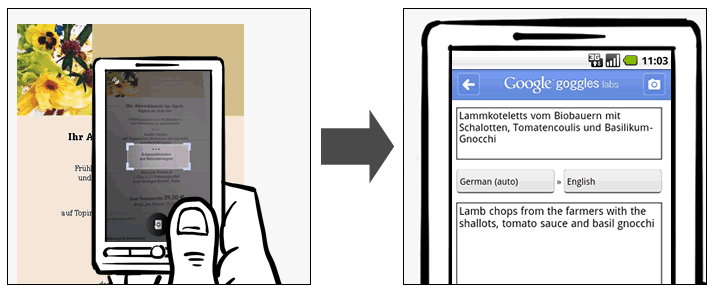
\includegraphics[scale=0.5]{google_goggles.png}
	\caption{Przykłd działąnia aplikacji Google Goggles\cite{googlegoggles}. }\label{fig:google_goggles}
\end{figure}

Aplikacja ta korzysta z usługi o tej samej nazwie dostarczanej przez korporacje Google. Usługa ta nie jest publicznie dostępna dlatego żadne bardziej szczegółowe informacje na jej temat nie są dostępne, lecz można się domyślać, iż integruje ona w sobie inne usługi dostarczane przez korporacje takie jak Google Translate czy Google Docs OCR. 

\section {Oddcast Illustrated Characters}

Oddcast Illustrated Characters\cite{oddcasts} jest to usługa integrująca w sobie funkcjonalność TTS i translację. Ciekawy jest sposób prezentacji wyników przetwarzania. Usługa udostępnia zestaw konfigurowalnych awatarów, które można dodać do strony internetowej albo aplikacji mobilnej. Następnie przy użyciu odpowiedniego API lub wbudowanego interfejsu użytkownika można wpisać tekst, wybrać odpowiedni język źródłowy i docelowy, a wynik przetwarzania będzie wypowiedziany przez awatara.

\begin{figure}[!h]
	\centering
	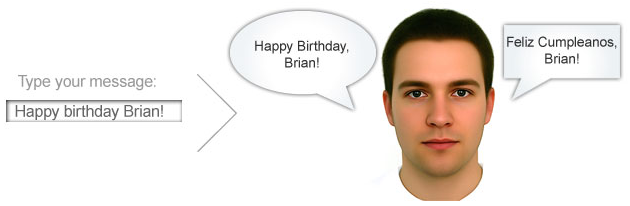
\includegraphics[scale=0.60]{oddcast.png}
	\caption{Przykład działania awatara Oddcast\cite{oddcasts}. }\label{fig:oddcast}
\end{figure}

Usługa ta jest bardzo prosta w integracji. Podstawowa integracja sprowadza się do wygenerowania odpowiedniego fragmentu kodu który należy dodać do swojej aplikacji. Obsługiwane technologie to Flash i JavaScript. Tyle wystarczy aby umożliwić użytkownikowi końcowemu używanie usługi do odsłuchiwania tłumaczonego tekstu. Dodatkowo, dostępne jest API, które daje większą kontrolę nad awatarem oraz procesem przetwarzania. 

Usługa ta integruje własnościowy syntezator mowy, który również jest dostępny jako osobna usługa. Na stronie producenta nie ma żadnych informacji na temat zastosowanego silnika translacji oraz na temat zastosowanej technologii integracyjnej.

\section {Pediaphon} 

Pediaphon\cite{pediaphon} jest aplikacją integrującą funkcjonalność TTS razem z darmową encyklopedią internetową: Wikipedia. Użytkownik podaje frazę, która zostaje wyszukana przy użyciu encyklopedii Wikipedia, a wynik wyszukiwania zostaje zamieniony na dźwięk. Użytkownik ma również opcję ustawienie parametrów przetwarzania, takich jak jakość i prędkość generowanej mowy oraz format wyjściowy. Aplikacja jest dostępna w różnych wersjach językowych w postaci strony internetowej oraz aplikacji na platformy mobilne: iPhone, Android. Do syntezy mowy aplikacja wykorzystuje silnik eSpeak razem z zestawem głosów MBROLA. eSpeak jest otwartym, programowym syntezatorem mowy dostępnym w postaci bibliotek lub narzędzia wiersza poleceń. Jakość generowanego dźwięku jest znacznie gorsza od komercyjnych rozwiązań takich jak IVONA.

\section*{Podsumowanie} 
Jak widać, zaprezentowane wyżej aplikacje prezentują różne scenariusze użycia. Najpoważniejsze ich wady to: ograniczona funkcjonalność, zamknięty interfejs, brak możliwości kontroli nad jakością generowanego dźwięku oraz brak interfejsu umożliwiającego ponowne wykorzystanie. System, którego projekt jest opisany w następnych rozdziałach, stara się  rozwiązać wszystkie wymienione problemy. Co więcej mógłby on całkowicie lub częściowo (usługi przetwarzania mowy) zastąpić każdą z wyżej wymienionych aplikacji. 
%\section {ReadSpeaker}




% ---------------------------------------------------------------------------
%: ----------------------- end of thesis sub-document ------------------------
% ---------------------------------------------------------------------------

